\Needspace{10\baselineskip}
\section{HDMI 视觉预处理流水线}
\label{sec:vision}
视觉预处理流水线为全自研 Verilog-2001 RTL，目标 720p60，流水线结构见图~\ref{fig:video}。

\begin{figure}[H]\centering
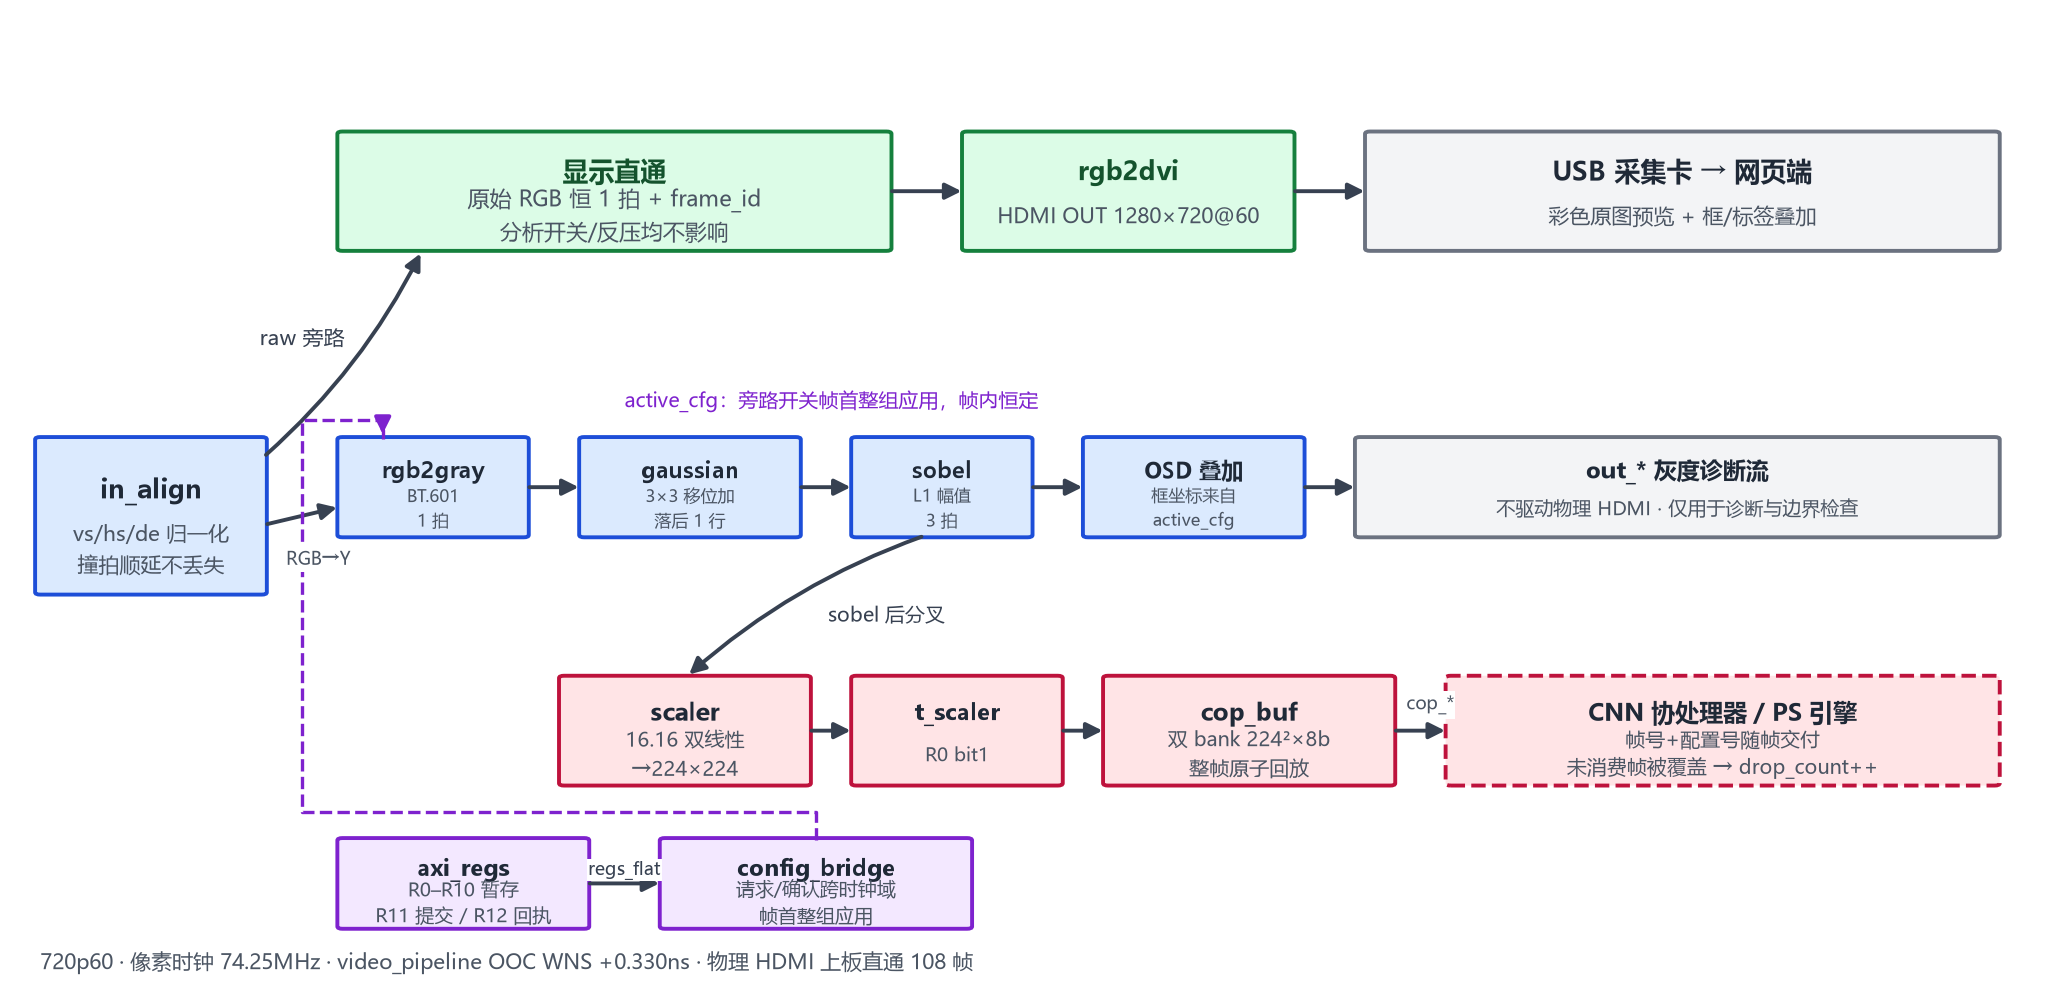
\includegraphics[width=0.98\linewidth]{fig_video.png}
\caption{视觉流水线三路径：显示直通、灰度分析与快照推理（仓库配图）}\label{fig:video}
\end{figure}

\subsection{流水线组成}
链路为 HDMI 接收（\code{dvi2rgb}）、输入对齐、高斯滤波、Sobel 边缘、缩放（scaler）与乒乓缓冲（\code{cop_buf}）。
配置寄存器采用原子配置契约：配置项成组提交、成组生效，避免运行中半新半旧的中间状态。
板上未搭载 ADV7611 器件，HDMI 接收采用 \code{dvi2rgb}/\code{rgb2dvi} 方案。

\subsection{显示与分析分流}
视频与分析路径在 RTL 内分流：
彩色原图以恒定延迟直通 \code{display_*} 口，用于 HDMI OUT 显示，保留原始色彩；
分析路径独立输出灰度 \code{out_*} 口，供定位与推理使用，坐标映射回显示画面。
该分流保证显示帧率不受分析耗时影响，也保证分析用的像素与训练采集的像素同源。

\subsection{时序收敛}
各单元 OOC 综合结果见表~\ref{tab:visiontiming}。
scaler 初版 57.5 MHz 的主因为 lerp 乘法的 9 级进位链；切拍重排读调度后达 94.9 MHz，720p60 全链正裕量。
\code{video_pipeline} 整体 OOC WNS +0.330 ns（2026-10-27 口径）。

\begin{table}[H]\centering\small
\caption{视觉单元 OOC 时序（OOC 综合口径）}\label{tab:visiontiming}
\begin{tabularx}{\linewidth}{@{}P{40mm}P{34mm}Y@{}}\toprule
单元 & 频率口径 & 备注\\\midrule
处理单元 & 约 88 MHz & 初版 OOC\\
高斯/Sobel & 约 76 MHz & 初版 OOC\\
scaler（初版） & 57.5 MHz & lerp 乘法进位链\\
scaler（切拍重排后） & 94.9 MHz & 720p60 全链正裕量\\
\code{video_pipeline} 整体 & WNS +0.330 ns & 2026-10-27 口径\\\bottomrule
\end{tabularx}\end{table}

\subsection{验证}
视觉 RTL 配有 22 个仓库内 tb（2026-10-27 口径），当前脚本入口以 \code{sim/scripts} 为准。
六套黄金参考与 RTL 输出逐像素对拍，误差不超过 2 LSB。
XSim 与 Icarus 双工具对拍，交叉排除仿真器差异。
物理 HDMI 板级直通实测 108 帧稳定输出（2026-10-03 上板记录）。
数据采集规程规定数据集必须经板卡 \code{hdmi_in.readframe()} 采集，保证数据集像素与部署像素一致。
\FloatBarrier
